\documentclass[10pt,a4paper,titlepage]{article}
\usepackage[utf8]{inputenc}
\usepackage[spanish]{babel}
\usepackage{amsmath}
\usepackage{amsfonts}
\usepackage{amssymb}
\usepackage[left=3cm,right=2cm,top=2.5cm,bottom=2.5cm]{geometry}
\usepackage{graphics,graphicx, float} %para incluir imágenes y colocarlas
\newcommand{\horrule}[1]{\rule{\linewidth}{#1}} % Create horizontal rule command with 1 argument of height
\usepackage[hidelinks]{hyperref} % Estilo para los enlaces
\hypersetup{
  colorlinks   = true, %Colours links instead of ugly boxes
  urlcolor     = blue, %Colour for external hyperlinks
  linkcolor    = black, %Colour of internal links
  citecolor   = blue %Colour of citations
}
\usepackage{url} % ,href} %para incluir URLs e hipervínculos dentro del texto (aunque hay que instalar href)


%----------------------------------------------------------------------------------------
%	TÍTULO Y DATOS DEL ALUMNO
%----------------------------------------------------------------------------------------


\date{\normalsize\today} % Incluye la fecha actual


\begin{document}
\begin{center}
{\Huge \emph{DS - Apuntes - Tema 1} } \\
\vspace{0.5cm}
Autor: Jose Luis Martínez Ortiz\\
\horrule{2pt} \\[0.5cm] % Thick bottom horizontal rule
\vspace{1.5cm}
\end{center}


\date{\normalsize\today} % Incluye la fecha actual
\tableofcontents % para generar el índice de contenidos

\newpage

\section{Introducción de UML}
\subsection{Diagrama de Clases}
Un diagrama de clases UML contiene una serie de elementos que detallaremos a continuación, pero podemos distinguirlos claramente en dos tipo, Objetos y relaciones.
Los objetos son una representación de un ente que queremos representar en el módelo UML, como por ejemplo un \textit{empleado} en un sistema software de una empresa o un \textit{vehículo}. Las relaciones se pueden dar entre dos objetos, estos dos objetos pueden ser el mismo pero es un caso un poco especial.\\

\subsubsection{Objetos}
Los objetos los identificaremos como clases y siguen el esquema de la figura \ref{fig:uml_clase}, donde podemos observar una una caja con 4 filas.

\begin{figure}[H] %con el [H] le obligamos a situar aquí la figura
\centering
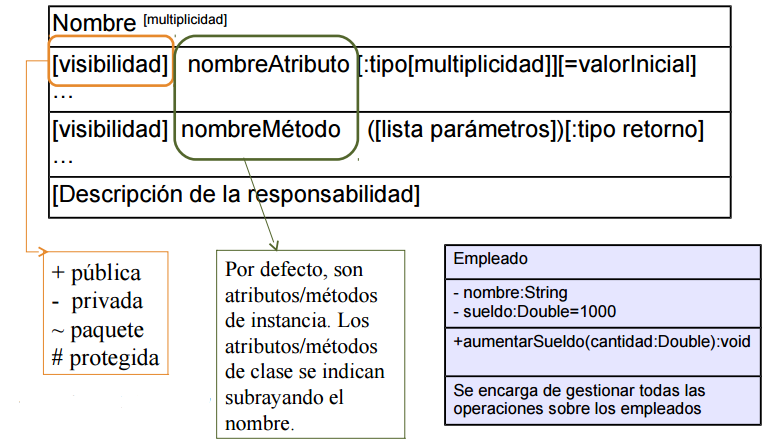
\includegraphics[scale=0.6]{img/uml_clase.png}  %el parámetro scale permite agrandar o achicar la imagen. En el nombre de archivo puede especificar directorios
\caption{Esquema de una clase uml} \label{fig:uml_clase}
\end{figure}

En la primera fila se indica el nombre del objeto que se va a modelar, así como su multiplicidad (singleton, interface, abstracta, etc).\\

En la segunda y tercera fila se indican los atributos y métodos respectivamente,  que definen al objeto, para ello indicamos:
\begin{enumerate}
\item \textbf{visibilidad :} indica cual es la ``privacidad'' del atributo.
	\begin{itemize}
	\item \textbf{+} : significa que el atributo o método es público y puede ser visto y utilizado por todo el mundo que tenga acceso a al objeto.
	\item \textbf{-} : significa que el atributo o método es privado y que solo el propio objeto puede verlo y utilizado.
	\item \textbf{$\sim$} : significa que el atributo o método es de paquete y solo los objetos que pertenecen al mismo paquete pueden acceder al el, es decir, es público dentro del paquete al que pertenece y es privado para todos los demás.
	\item \textbf{\#} : significa que el atributo o método es protegido y solo el mismo y sus descendientes pueden verlo y utilizarlo.
	\end{itemize}

\item \textbf{nombre} : del atributo o del método. Puede ser de clase si van subrayados. Los métodos/atributos de instancia están asociados a los objetos cuya invocación se realiza mediante envío de mensajes entre objetos y los métodos/atributos de clase Son métodos asociados a la clase que se pueden invocar sin necesidad de crear ninguna instancia (ningún objeto). Por ejemplo en java se definen con la palabra ``\texttt{static}''

\item \textbf{Tipo} : clase a la que pertenece ese atributo.
\item \textbf{lista de parámetros} : conjunto de nombre\_atributo:tipo.
\item \textbf{multiplicidad de atributo} : número de elementos en dicho atributo.
\item \textbf{valor inicial} : indica el valor por defecto de dicho atributo.
\item \textbf{tipo retorno} : indica el tipo de objeto que devuelve.

\end{enumerate}

En la cuarta fila se hace una breve descripción de la responsabilidad de dicho objeto.
Principalmente se utilizan los tipos de clases: Normal, Abstracta e Interfaz.\\

\underline{\textbf{Abstracción}}\\
Una clase abstracta es una clase que no se puede instanciar y se usa únicamente para definir subclases. Las clases abstractas siempre tiene que tener al menos un método sin implementar. Se deben de utilizar para implementar algunos métodos pero dejando otros para las subclases.
El nombre de la clase aparece en cursiva. Los métodos abstractos (no implementados)
aparecen en cursiva. Una clase abstracta debe ser heredada por subclases. La cabecera de un método de una clase abstracta debe coincidir en las subclases que lo heredan. La
visibilidad puede modificarse en las subclases siempre que sea a mayor. También el tipo de retorno, que puede ser un subtipo en las subclases.\\

\underline{\textbf{Interfaz}}\\
Básicamente es una clase abstracta pero que todos los métodos son abstractos, es decir que o se implementan todos los métodos o ninguno. Su utilización también es para la de indicar unas ``reglas'' que debe de cumplir una clase.
\begin{figure}[H] %con el [H] le obligamos a situar aquí la figura
\centering
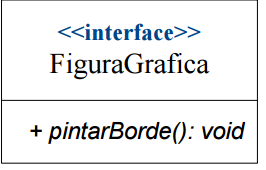
\includegraphics[scale=0.6]{img/uml_interfaz.png}
\caption{Ejemplo una clase interfaz.} \label{fig:uml_interfaz}
\end{figure}

\subsubsection{Relaciones}
Las relaciones entre objetos pueden ser de muchísimas formas y con múltiples significados para poder modelar todas las opciones que se plantean a la hora de diseñar un software. Se van a describir a continuación las principales relaciones entre dos objetos.\\

Vamos a definir también los elementos de las asociaciones y un ejemplo:
\begin{itemize}
\item \textbf{Nombre:} Nombre de la asociación. Se puede indicar hacia dónde se lee empleando el símbolo $\blacktriangleright$.
\item \textbf{Rol:} Se emplea para explicitar el papel que juega cada clase en la asociación.
\item \textbf{Navegabilidad:} Representa si el conocimiento entre los objetos de los extremos de la asociación es unidireccional ($\rightarrow$ o $\leftarrow$) o bidireccional (sin punta de flecha en ninguno de los extremos).
\item \textbf{Multiplicidad:} Indica el número de objetos de una clase
que pueden asociarse con un objeto de la otra clase. Su sintaxis es \texttt{valorMínimo..valorMáximo}, pudiendo usarse * para especificar ``varios'' y así no dar un valor máximo concreto. Si no se indica nada, por defecto es 1.
\end{itemize}
\begin{figure}[H] %con el [H] le obligamos a situar aquí la figura
\centering
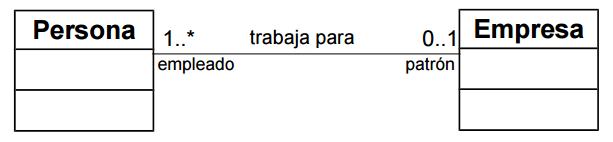
\includegraphics[scale=0.6]{img/uml_relacion_elementos.png}
\caption{Ejemplo de los elementos de una relación.} \label{fig:uml_rel_elementos}
\end{figure}

\underline{\textbf{Dependencia}}\\
Modelan una relación débil y poco duradera en el tiempo, se representa con una fecha con una linea de puntos hacia el objeto que necesita. Significa que en algún momento se requerirá al objeto relacionado para momentos muy concretos, siendo la vida de esta relación normalmente de ámbito de método. En la figura \ref{fig:uml_rel_dependencia}
\begin{figure}[H] %con el [H] le obligamos a situar aquí la figura
\centering
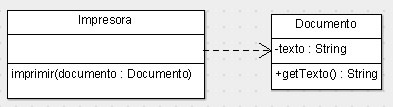
\includegraphics[scale=0.6]{img/uml_relacion_dependencia_ejemplo.png}
\caption{Ejemplo de una relación de dependencia.} \label{fig:uml_rel_dependencia}
\end{figure}

\underline{\textbf{Asociación}}\\
Modela una relación estructural fuerte y duradera en el tiempo (figura \ref{fig:uml_rel_asociacion} ).
\begin{figure}[H] %con el [H] le obligamos a situar aquí la figura
\centering
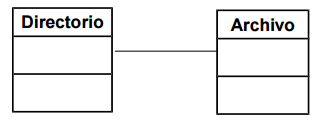
\includegraphics[scale=0.9]{img/uml_relacion_asociacion_ejemplo.png}
\caption{Ejemplo de una relación de asociacion.} \label{fig:uml_rel_asociacion}
\end{figure}

Dentro de la asociación encontramos también dos tipos especiales de relaciones que nutren a esta relación de más significado, como es la ``Agregación'' y la ``Composición''. \\

La \textit{Agregación} es una asociación cuyo nombre es ``parte de'', en la que una de las clases representa el ``todo'' y la otra la/s ``parte/s'', es decir, ambos objetos tiene sentido por si mismos pero uno de ellos es parte del otro. Se representa con un rombo blanco en el extremo de la relación.\\
\begin{figure}[H] %con el [H] le obligamos a situar aquí la figura
\centering
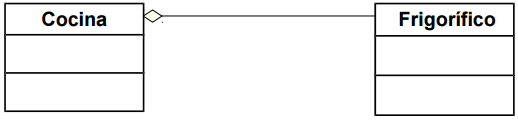
\includegraphics[scale=0.7]{img/uml_relacion_agregacion.png}
\caption{Ejemplo de una relación de asociacion - agregación.} \label{fig:uml_rel_agregacion}
\end{figure}

La \textit{Composición} es como una agregación fuerte, en que la/s parte/s no tiene/n sentido sin el todo. Se representa como un rombo negro en el extremo de la relación. Se puede decir que ambas partes están incompletas sin la otra.
\begin{figure}[H] %con el [H] le obligamos a situar aquí la figura
\centering
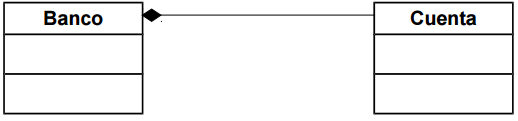
\includegraphics[scale=0.7]{img/uml_relacion_composicion.png}
\caption{Ejemplo de una relación de asociacion - composición.} \label{fig:uml_rel_composicion}
\end{figure}

\underline{\textbf{Herencia}}\\
La herencia en UML se representa como una relación entre dos clases y se denota con un
triangulo al final de la relación. En las subclases, sólo se indican las variables y los métodos nuevos que declaran. También se indican los métodos que, aunque figuren en la superclase, se redefinen en la subclase. 
\begin{figure}[H] %con el [H] le obligamos a situar aquí la figura
\centering
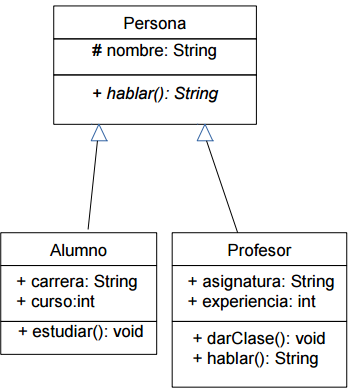
\includegraphics[scale=0.7]{img/uml_relacion_herencia.png}
\caption{Ejemplo de una relación de Herencia.} \label{fig:uml_rel_herencia}
\end{figure}

La relación de Herencia también se define en dos subtipos, generalización y especialización. En la generalización se identifican rasgos comunes entre varios tipos de entidad y se crea una superclase para todos ellos. Por ejemplo (figura \ref{fig:uml_rel_generalizacion}) los tipos de entidad COCHE y CAMIÓN de la izquierda se generalizan a la derecha en la superclase VEHÍCULO con los atributos comunes. Se está realizando un refinamiento bottom-up o ascendente.
\begin{figure}[H] %con el [H] le obligamos a situar aquí la figura
\centering
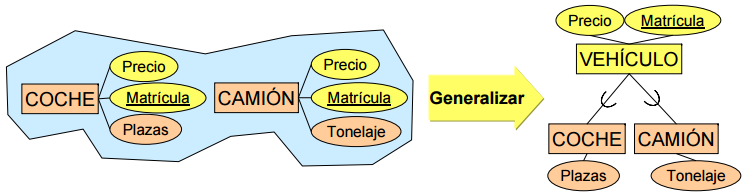
\includegraphics[scale=0.7]{img/uml_relacion_generalizacion.png}
\caption{Ejemplo de una relación de Herencia por Generalización.} \label{fig:uml_rel_generalizacion}
\end{figure}

Es el proceso de dividir un tipo de entidad en subclases. Es lo contrario a generalizar: aquí el refinamiento es top-down o descendente. Un conjunto de subclases se define a partir de alguna característica distintiva. Podemos tener varias especializaciones sobre el mismo tipo de entidad:\\
– Por tipo de trabajo: Secretario, Técnico, Gerente\\
– Por método de pago: Asalariado, Por horas

\begin{figure}[H] %con el [H] le obligamos a situar aquí la figura
\centering
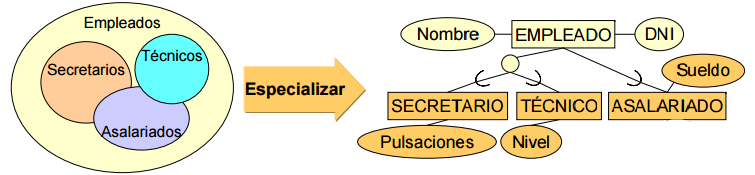
\includegraphics[scale=0.6]{img/uml_relacion_especializacion.png}
\caption{Ejemplo de una relación de Herencia por Especialización.} \label{fig:uml_rel_especializacion}
\end{figure}


\underline{\textbf{Realización}}\\
La realización es una relación que indica que la clase va a realizar una implementación de la clase interfaz a la que apunta. Se simboliza como una linea discontinua acabada en un triangulo. La clase que tiene una realización sobre la interfaz esta obligada a implementar los métodos de esta.
\begin{figure}[H] %con el [H] le obligamos a situar aquí la figura
\centering
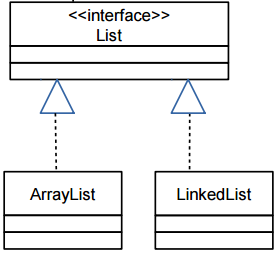
\includegraphics[scale=0.6]{img/uml_relacion_realizacion.png}
\caption{Ejemplo de una relación de realización.} \label{fig:uml_rel_realizacion}
\end{figure}






\end{document}










